

\documentclass[11pt]{article} 

\usepackage[utf8]{inputenc} 

\usepackage{amsmath}
\usepackage[polish]{babel}
\usepackage{geometry}
\geometry{a4paper} 

\usepackage{polski}
\usepackage{url}
\frenchspacing
\usepackage{graphicx} 
\usepackage{booktabs} 
\usepackage{array}
\usepackage{paralist}
\usepackage{verbatim} 
\usepackage{subfig} 


\usepackage{fancyhdr} 
\pagestyle{fancy} 
\renewcommand{\headrulewidth}{0pt} 
\lhead{}\chead{}\rhead{}
\lfoot{}\cfoot{\thepage}\rfoot{}

\usepackage{sectsty}
\allsectionsfont{\sffamily\mdseries\upshape} 
\usepackage[nottoc,notlof,notlot]{tocbibind} 
\usepackage[titles,subfigure]{tocloft} 
\renewcommand{\cftsecfont}{\rmfamily\mdseries\upshape}
\renewcommand{\cftsecpagefont}{\rmfamily\mdseries\upshape} 

\title{Porównanie działania algorytmów wyszukiwań w grafie}
\author{Karolina Morawska}
%\date{} % Activate to display a given date or no date (if empty),
         % otherwise the current date is printed 

\begin{document}

\maketitle
\newpage
\tableofcontents
\newpage
\section{Czym wogóle jest graf ?}
 To taka struktura danych, która składa się z wierzchołków i krawedzi, przy czym poszczególne wierzchołki (zwane też węzłami) mogą być połączone krawędziami (skierowanymi lub nieskierowanymi) w taki sposób, iż każda krawędź zaczyna się i kończy w którymś z wierzchołków. Wierzchołki i krawędzie mogą być numerowane, etykietowane i nieść pewną dodatkową informację - w zależności od potrzeby modelu, do którego konstrukcji są wykorzystane. W porównaniu do drzew w grafach mogą występować pętle i cykle. Krawędzie mogą mieć wyznaczony kierunek (wtedy graf nazywamy skierowanym), mogą mieć przypisaną wagę (pewną liczbę), kolor, etykietę, np. odległość pomiędzy punktami w terenie, rodzaj połączenia.

  \begin{figure}[ht!] 
\centering
 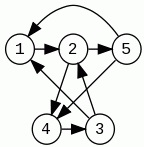
\includegraphics[width=70mm]{grafsk}
 \caption{Przykład grafu skierowanego} 
\label{overflow}
 \end{figure}
Istnieje wiele rodzajów grafów, które mogą mieć wiele interesujących właściwości. Grafy mogą być, np.:

\begin{itemize}
\item Skierowane gdy możliwe jest przejście pomiędzy wierzchołkami tylko w jedną stronę (krawędź wtedy oznaczamy strzałką).
\item Nieskierowane gdy możliwe jest przejście pomiędzy wierzchołkami w obydwie strony.
\end{itemize}
Naszym zadaniem było zaimplementowanie grafu nieskierowanego.
\newpage
\subsection{Opis implementacji grafu nieskierowanego wybranego przeze mnie.}

Wybrałam implememtacje grafu za pomocą listy sąsiedztwa.Reprezentacja grafu za pomocą list sąsiedztwa jest podobna do reprezentacji macierzą sąsiedztwa. Mamy tablicę n-elementową, gdzie n oznacza liczbę wierzchołków w grafie. Każdy element tej tablicy jest skojarzony z jednym wierzchołkiem grafu - numer wiersza jest numerem wierzchołka. Elementy tablicy są listami. Listy te zawierają numery wierzchołków w grafie, do których prowadzi z danego wierzchołka krawędź.
\\Zaletą takiej implementacji jest:
\begin{itemize}
\item  Oszczędność pamięci komputera, ponieważ odwzorywane są  tylko istniejące krawędzie.
\item Dostęp do sąsiadów danego wierzchołka jest szybszy niż w przypadku tablicy sąsiedztwa, ponieważ nie musimy sprawdzać kolejnych wierzchołków - lista od razu zawiera gotowych do odczytu sąsiadów.
\end{itemize}
  \begin{figure}[ht!] 
\centering
 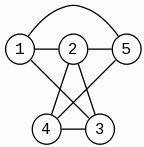
\includegraphics[width=70mm]{graf}
 \caption{Przykład grafu nieskierowanego} 
\label{overflow}
 \end{figure}
\newpage
\section{Algorytmy służące do przeszukiwania grafu}
\subsection{Breadth-first search, czyli przeszukiwanie wszerz}
Jest to jeden z najprostszych algorytmów przeszukiwań służacy do odnajdywania najkrótszej drogi w grafie. Przechodzenie grafu rozpoczyna się od zadanego wierzchołka i polega na odwiedzeniu wszystkich dostępnych z niego wierzchołków.

\underline{Złożoność pamięciowa}

 Algorytmu uzależniona jest od sposobu implementacji grafu.W moim przypadku czyli implementacji grafu za pomocą listy sąsiedztwa dla każdego wierzchołka przechowywana jest lista wierzchołków dostępnych bezpośrednio z niego.Złożoność pamięciowa wynosi $O(|V|+|E|)$ gdzie$|V|$ to liczba węzłów a $|E|$ to liczba krawędzi w grafie.
 
\underline{Złożonośc czasowa}

Ponieważ w najgorszym przypadku przeszukiwanie wszerz musi przebyć wszystkie krawędzie prowadzące do wszystkich węzłów, złożoność czasowa tego przeszukiwania wynosi$ O(|V| + |E|)$, gdzie $|V|$ to liczba węzłów, a $|E|$ to liczba krawędzi w grafie.

\subsection{Depth-first search, czyli przeszukiwanie w głąb}
Polega na badaniu wszystkich krawędzi wychodzących z podanego wierzchołka.Po zbadaniu wszystkich krawędzi wychodzących danego wierzchołka algorytm powraca do wierzchołka, z którego dany wierzchołek został odwiedzony.

\underline{Złożoność pamięciowa} 

Algorytmu w przypadku drzewa jest o wiele mniejsza niż przeszukiwania wszerz, gdyż algorytm w każdym momencie wymaga zapamiętania tylko ścieżki od korzenia do bieżącego węzła, podczas gdy przeszukiwanie wszerz wymaga zapamiętywania wszystkich węzłów w danej odległości od korzenia, co zwykle rośnie wykładniczo w funkcji długości ścieżki.

\underline{Złożoność czasowa} 
Przeszukiwania jest uzależniona od liczby wierzchołków oraz liczby krawędzi. Algorytm musi odwiedzić wszystkie wierzchołki oraz wszystkie krawędzie, co oznacza, że złożoność wynosi $O(|V|+|E|)$.
\newpage
\subsection{Algorytm A*}
 Jego zadaniem jest znalezienie najkrótszej ścieżki między dwoma węzłami grafu.Został opracowany w 1968r . przez N.Nilssona oraz B.Raphaela. Jest to algorytm zupełny i optymalny, ponieważ znajduje ścieżke, jeśli taka istnieje i przy tym jest to ścieżka najkrótsza.Wykorzystywany często w grach komputerowych do wyznaczania tras przejścia obiektu między dwoma punktami w grze.

Algorytm A* szuka najkrótszej drogi łączącej pole startowe z docelowym, zaczynając od sprawdzenia pól (jakie są w otoczeniu punktu, w którym znajduje się algorytm oraz które jeszcze nie były rozpatrywane), przez które prowadzą potencjalnie najbardziej obiecujące drogi do celu. Jest to zachowanie właściwe dla algorytmów typu „Best-first search”, opartych na zasadzie rozpatrywania w pierwszej kolejności (potencjalnie) najwartościowszych przypadków. Jednakże algorytm A* nie posiada cech algorytmu zachłannego, gdyż przy poszukiwaniu najkrótszej drogi uwzględnia on długość (koszt) drogi od punktu startowego do punktu aktualnie rozpatrywanego. 

W omawianym algorytmie niezmiernie ważną rzeczą jest wybranie odpowiedniej funkcji heurystycznej  czyli funkcji h, która oblicza wartości parametru H dla poszczególnych punktów przestrzeni. Zastosowanie takiej funkcji h, która dla każdego pola przestrzeni nie doszacowuje faktycznej najkrótszej odległości pola od celu (czyli posługuje się taką wartością odległości od celu, że zawsze jest ona nie większa, niż odległość faktyczna), gwarantuje znalezienie optymalnego rozwiązania. W miarę wzrostu jakości oszacowania szybkość działania algorytmu A* rośnie (sprawdzana jest mniejsza liczba węzłów), natomiast w momencie, gdy zaadoptujemy funkcję heurystyczną przeszacowującą rzeczywistą odległość pól przestrzeni, to algorytm jeszcze bardziej ograniczy liczbę przeszukiwań (a tym samym ograniczymy czas jego działania), natomiast może to grozić nieznalezieniem rozwiązania optymalnego (choć otrzymany rezultat będzie najczęściej suboptymalny). Dlatego przy rzeczywistym zastosowaniu tego algorytmu np. w grze komputerowej warto zastanowić się, czy ważniejsza jest dla nas szybkość obliczeń (by był krótki czas oczekiwania na poruszenie się obiektu w grze), czy dokładność w wyznaczaniu najkrótszej drogi. 

\underline{Obliczeniowa złożoność czasowa}

Algorytmu A* zależy od zastosowanej heurystyki. W najgorszym przypadku liczba przeszukanych węzłów rośnie wykładniczo w stosunku do długości rozwiązania (najkrótszej ścieżki), natomiast rośnie już tylko wielomianowo, jeśli funkcja heurystyki h spełnia następujący warunek:

  \begin{math}  |h(x) - h^*(x)| = O(\log h^*(x))
  \end{math}
 - gdzie $h^*$ jest optymalną heurystyką, czyli zawsze podaje dokładny, rzeczywisty koszt ścieżki z x do węzła końcowego. Innymi słowy, błąd funkcji h nie powinien rosnąć szybciej niż logarytm "dokładnej heurystyki" $h^*$.
 \newpage
 \section{Przeprowadzone testy sprawdzające poprawość wyszkukiwań każdego z tych algorytmów.
 Zadaniem programu było znalezienie ścieżki z wierzchołka 1 do 4}

  \begin{figure}[ht!] 
\centering
 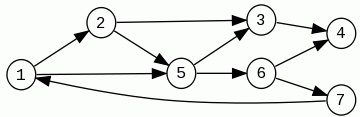
\includegraphics[width=120mm]{graphchart1}
 \caption{Pierwszy z grafów wykorzystany w testach} 
\label{overflow}
 \end{figure}
 Wyniki testów dla Grafu nr 1:
 
 A* :
 1$->$5$->$6$->$4 Czas wyszukiwania: 128 ns
 
 DFS:
 1$->$5$->$6$->$7$->$4 Czas wyszukiwania:  3960 ns
 
 BFS:
 1$->$2$->$3$->4$ Czas wyszukiwania:  4678 ns
 
 
  \begin{figure}[ht!] 
\centering
 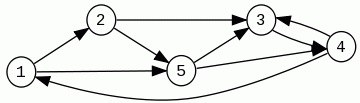
\includegraphics[width=120mm]{graphchart2}
 \caption{Drugi z grafów wykorzystany w testach} 
\label{overflow}
 \end{figure}
 Wyniki testów dla Grafu nr 2:
 
 A* :
 1$->$5$->$4$->$3 Czas wyszukiwania: 102 ns
 
 DFS:
 1$->$5$->$4$->$3 Czas wyszukiwania : 3850 ns
 
 BFS:
 1$->$2$->$3    Czas wyszkukiwania: 4420 ns
 
 \newpage
 \section{Wnioski i uwagi}
 \begin{itemize}
 \item Algorytm A* znajduje najkrótszą ścieżkę, zatem funkcja heurystyczna zwraca 0.Działa też o wiele szybciej dla dużej ilości wierzchołków i krawędzi niż pozostałe algorytmy.
 \item Duży wpływ na to który algorytm BFS , DFS lub A* pokaże lepszą ścieżke ma budowa grafu(ilość wierzchołków i krawędzi).
 \item Przy małych ilościach danych bardziej efektywniejsze są algorytmy BFS i DFS pod względem wydajności.
 \end{itemize}
  \newpage
\begin{thebibliography}{99}

\bibitem{pa}
\emph{$http://zasoby1.open.agh.edu.pl/dydaktyka/informatyka$}

\bibitem{pa}
\emph{$http://pl.wikipedia.org/wiki/Przeszukiwanie_wszerz$}

\bibitem{pa}
\emph{$http://pl.wikipedia.org/wiki/Przeszukiwanie_w$}

\bibitem{pa}
\emph{$http://www.algorytm.org/algorytmy$-$grafowe/przeszukiwanie$-$grafu$-$wszerz$-$bfs$-$i$-$w$-$glab$-$dfs.html$}

\bibitem{pa}
\emph{$http://iair.mchtr.pw.edu.pl/~bputz/aisd_cpp/lekcja7/segment4/main.htm$}
\end{thebibliography}
\end{document}

\end{document}
